%%%%%%%%%%%%%%%%%%%%%%%%%%%%%%%%%%%%%%%%%%%%%%%%%%%%%%%%
%
% Change the option between square brackets
% depending on the document you have to write:
%
% proposal    for the initial proposal
% review      for the literature review
% progress    for the progress report
% final       for the final 
% 
%%%%%%%%%%%%%%%%%%%%%%%%%%%%%%%%%%%%%%%%%%%%%%%%%%%%%%%%
\documentclass[final]{cmpreport}
\makeatletter
\input{t1pcr.fd}
\makeatother
\setlength{\footnotesep}{3ex}

% Some package I am using. You may not need them
%
\usepackage{rotating}
\usepackage{subfloat}
\usepackage{color}
\usepackage{amsmath}
\usepackage[linesnumbered,ruled,vlined]{algorithm2e}
\usepackage{float}
\usepackage[export]{adjustbox}
\usepackage{hyperref}

%\setkeys{Gin}{draft}

%%%%%%%%%%%%%%%%%%%%%%%%%%%%%%%%%%%%%%%%%%%%%%%%%%%%%%%%
%
%  Fill in the fields with:
%
%  your project title
%  your name
%  your registration number
%  your supervisor's name
%
%%%%%%%%%%%%%%%%%%%%%%%%%%%%%%%%%%%%%%%%%%%%%%%%%%%%%%%%
\title{Real-time Ray Tracing}
%%%%%%%%%%%%%%%%%%%%%%%%%%%%%%%%%%%%%%%%%%%%%%%%%%%%%%%%
%
% The author's name is ignored if the following command 
% is not present in the document
%
% Before submitting a PDF of your final report to the 
% project database you may comment out the command
% if you are worried about lack of anonimity.
%
%%%%%%%%%%%%%%%%%%%%%%%%%%%%%%%%%%%%%%%%%%%%%%%%%%%%%%%%
\author{Kiefer Lam}

\registration{100166387}
\supervisor{Dr Stephen Laycock}

%%%%%%%%%%%%%%%%%%%%%%%%%%%%%%%%%%%%%%%%%%%%%%%%%%%%%%%%
%
% Fill in the field with your module code.
% this should be:
%
% for BIS            -> CMP-6012Y
% for BUSINESS STATS -> CMP-6028Y
% for other students -> CMP-6013Y
%
%%%%%%%%%%%%%%%%%%%%%%%%%%%%%%%%%%%%%%%%%%%%%%%%%%%%%%%%
\ccode{CMP-6013Y}
%\ccode{CMP-6012Y / CMP-6013Y / CMP-6028Y}


\summary{
This document explains how to use the class file \texttt{cmpreport.cls} to write your reports.
The class file has been designed to simplify your life; many things are done for you. As a consequence
some commands presented here are specific to the class file whether they are new commands or customized versions
of commonly known \LaTeX\ commands.
}

\acknowledgements{
This section is used to acknowledge whoever's support and contribution.
The command that introduces it is ignored in the project proposal, literature review and progress report. It is used in the
final report,  but  is not compulsory. If you do not
have an acknowledgements command in your preamble then there
won't be any acknowledgement section in the document produced. \emph{Abstract} and \emph{Acknowledgements} sections should fit on the same page. 
}

%%%%%%%%%%%%%%%%%%%%%%%%%%%%%%%%%%%%%%%%%%%%%%%%%%%%%%%%%%%%%%%%%%
%
% If you do not want a list of figures and a list of tables
% to appear after the table of content then uncomment this line 
%
% Note that the class file contains code to avoid
% producing an empty list section (e.g list of figures) if the 
% list is empty (i.e. no figure in document).
%
% The command also prevents inserting a list of figures or tables 
% anywhere else in the document
%
% Some supervisors think that a report should not contain these
% lists. Please ask your supervisor's opinion.
%
%%%%%%%%%%%%%%%%%%%%%%%%%%%%%%%%%%%%%%%%%%%%%%%%%%%%%%%%%%%%%%%%%%
%\nolist

%%%%%%%%%%%%%%%%%%%%%%%%%%%%%%%%%%%%%%%%%%%%%%%%%%%%%%%%%%%%%%%%%%
%
% Comment out if you want your list of figures and list of
% tables on two or more pages, in particular if the lists do not fit 
% on a single page.
%
%%%%%%%%%%%%%%%%%%%%%%%%%%%%%%%%%%%%%%%%%%%%%%%%%%%%%%%%%%%%%%%%%%
\onePageLists

\begin{document}

\section{Introduction}

\subsection{Aims and Motivations}
Ray tracing has already been established as a viable technique to produce realistic graphics in computer generated graphics by simulating light rays. The aim for the project is to be able to produce visually realistic images quickly, sequentially, and continuously to create a real-time experience. A real-time application is subject to real-time constraints where the application must produce a response to an event within a time constraint. In this case, the application must produce an image in time after an event such as user input. There are many use cases for this project including:

\begin{itemize}
    \item Realistic visuals in 3D games
    \item Faster rendering for computer generated imagery in video
    \item Simulating light rays and how they interact with objects in a scene
\end{itemize}

\subsection{Problems}
Many industries already use the ray tracing technique to produce realistic visuals in games or video however the universal issue that comes with ray tracing is performance. Since the technique requires a significant number of rays to produce a realistic and accurate (not noisy) image, it often takes a long time for the rendering process. There is usually a trade-off between visual fidelity and performance \citep{RTPerfEnergyCost}. 
\paragraph{Video}
Real time ray tracing is less of a problem for video as the experience is not affected by the speed at which the video was rendered. Because of this, ray tracing in CGI uses more rays to create a more realistic image. However it would still benefit from performance during production. 
\paragraph{Games}
Video games are an example of something that would benefit more from real-time ray tracing rendering as the experience is generally better and smoother when the image is rendered quicker. Games prioritise performance over realism as the game would be 'unplayable' if it is unable to produce the image with a quick response to user input. This is why games will usually use less rays at the expense of realism.

The number of rays is not the only factor affecting performance. Each individual ray has to perform an intersection test with every object in the scene. Simple objects such as spheres and planes will only require a single intersection test however complex models will require multiple intersection tests for each part of the model.

\section{Literature Review}
\subsection{Project: Real-time ray tracing}
\subsubsection{Brief}
In this report, I will discuss the ray tracing technique, its use in the project, the differences with rasterization, and the approaches to be used in the project.

\subsubsection{What is ray tracing?}
\paragraph{Computer Generated Image} Ray tracing is a technique used to computer graphically generate a 2D image of a 3D world typically viewed on a flat screen. The technique is commonly used to produce a high degree of visual realism in computer generated images.

\paragraph{Conventional Rendering Technique} Since ray tracing is relatively computationally intensive, rasterization is the conventional rendering technique used in mediums that require images to be rendered quickly with low response times to user input (low latency) such as video games. Rasterization generates the 2D image of the 3D world by projecting the fragments computed from a mesh with vertices and faces onto a plane which is then displayed onto the screen. However, ray tracing simulates the real world physical process of how objects are illuminated by light rays in a virtual world. To produce an image with high visual fidelity, an innumerable amount of rays must be used. Depending on the complexity of the scene, millions of rays may have to be generated to produce a single image.

\paragraph{Realtime-ness} For the project to run in real-time, the system must guarantee response to events with low latency. The latency of the response must be in the order of milliseconds for the system to be real-time; more so in applications such as video games where a high response time will result in a complete failure as a game. An example in a video game would be: the user inputting an event to move a character and the response being the system displaying an image with the character in a different location appearing to move. The realtime-ness of the application will largely depend on the time it takes for the image to be rendered as it is the main process causing the latency.

\paragraph{Ray tracing approach} To produce the image, a ray is created for each pixel of the image. These initial rays are referred to as primary rays and are traced outwards from the camera origin. This approach is modelled after the pinhole camera where light rays pass through the pinhole and land on the film (screen) at the location corresponding to the angle of the ray \citep[1.1.2]{introraytracing}. It would be unreasonable to simulate this by tracing all light rays originating from every light source and capturing the light rays that happen to land on the screen. This is forward ray tracing. Instead, we would use backward ray tracing the rays are traced from the screen and towards a light source \citep[1.2]{introraytracing}. The light sources may sometimes be other objects and not necessarily a true light source and the bounces of rays are usually limited to a relatively small number (relative to the true actual number of bounces of light rays in the real world). The purpose of these limits are to impose a time constraint so that the result is produced in a reasonable time frame making it smoother. This will reduce the potential degree of realism that can be achieved however it is necessary to ensure the system runs in real-time. The most basic ray tracer would return the colour of the closest object hit by the primary ray which would apply as the colour of the pixel for the ray. However this does not produce a very realistic image; more rays must be traced, originating from the intersection point, to create a more realistic image with lighting and shadows.

\paragraph{Secondary rays} Rays stemming from the intersection point of the primary ray are referred to as secondary rays. Lighting, shadows, reflection, and refraction are some of the features that can be simulated with secondary rays. When the primary ray intersects with an object, more rays can be generated with the intersection point as the origin. The direction of the ray may be different depending on the information we are trying to find. Secondary rays can be generated and processed recursively to simulate light bounces.

\paragraph{Shadow rays} To determine whether the primary ray intersection point is in a shadow, a secondary ray can be generated and traced towards light sources where the point would be in a shadow if it intersects with an object before the light source. The result from the primary ray can then be modified to make the pixel appear darker and in effect, in the shadow.

\paragraph{Reflections} When reflection rays are generated, the direction of the new ray should be reflected about the normal of the surface of the intersection point. The outward angle from the normal should be the same as the angle of incidence of the previous ray. The new ray can be treated as a primary ray and have its result mixed with the parent ray with varying degrees depending on the reflectivity of the objects material. For example, a mirror would have more weight on the colour value of the reflection ray than the primary/parent ray. 

\paragraph{Refraction} The basic idea of tracing refraction is also based on refraction in the real world where physical concepts are considered instead of brute force tracing the ray, stepping through the object until the ray exits. If the object material information has a refractive index, we can use this information and the angle of incidence to find the angle at which the light ray \lq{}travels\rq{} through the object. This method assumes the density of the object is constant.

\paragraph{Combining rays} \citep[1.2.3]{introraytracing} To determine the colour of the pixel, we have to combine all the rays that the pixels corresponding primary ray and all of its secondary rays to produce a sensible colour to be displayed on the screen. For example, a red and green ray should combine and produce the colour yellow. We also have to take into account that light rays usually lose energy when they bounce around in the real world. This can be achieved by reducing the weight of a rays impact on the final result depending on the number of bounces before the secondary ray. Shadows, reflections, and refractions will require different algorithms for combining their results into the final result. Physically, these are all the same type of ray, but it is convenient to classify them as different rays computationally. The combining algorithm will be more complex than it may seem at first. When real world physical light rays combine, their waves and amplitude superpose in an additive manner. If we apply that simple additive method to the ray tracer, we would end up with white most of the time as we add the ray colours and get values above 1.0 in the RGB channels. We could increase the dynamic range of the rays by using the highest value in the scene and use that as the ceiling, scaling every other value down proportionally. However this requires every pixel to be traced beforehand.

\paragraph{Aliasing} \citep[1.4]{introraytracing} The signal our eyes receive from light rays are continuous. There are no pixels or grids in the human eye so everything we see is smooth with great detail. The issue with modern computers is that they cannot represent a continuous signal. Digital images are made up of a grid of pixels where the size of a single pixel is the limit of how fine of a detail we can display. Because of this, the image produced will have an aliasing effect where a smooth edge appears jagged. To counter this, anti-aliasing techniques are used. One approach of anti-aliasing is tracing multiple primary rays per pixel where pixels are split into sub-pixels. This is referred to as multi-sampling (multiple samples for each pixel) and the final result of the pixel is a combination of the sub-pixels. The easiest way to achieve this would be to just produce an image with a higher resolution and scale it down when finally displaying the image, letting the display software decide on how to interpolate the neighbouring pixels. While it is the easiest and simplest approach, it is also the least efficient; there are more optimised techniques to achieve anti-aliasing faster and sometimes better. Instead of blindly tracing extra rays from each pixel, we can select the only the pixels which reside on the edges of objects to trace the sub-pixel rays as surfaces generally do not need anti-aliasing.

\subsubsection{Essential Algorithms}
\paragraph{Ray intersection algorithms} In order to detect whether a ray hits an object in the scene, we'll need to test whether the ray, as a straight line, intersects with the object. With only the ray-triangle intersection test, we can test every and any arbitrary shape as the shapes can just be converted into a triangle mesh. However this is inefficient as models and meshes could have a large number of triangles so it is a good idea to include tests for commonly used shapes such as spheres and planes.

\[ R = R_o + t(R_d) \]

The ray \( R \) is denoted by the ray origin \( R_o \) plus the ray direction \( R_d \) where \(R_o\) and \(R_d\) consist of three components \((x, y, z)\). Any point on the ray can be calculated by adjusting \(t\) where \(t > 0 \). For values of \(t < 0\), the point is behind the ray origin and therefore disregarded.

\paragraph{Spheres} \citep{linesphereintersect} Spheres are commonly used in ray tracing to test the ray tracing techniques as the every point on the surface of a sphere has a different normal. The intersection test algorithm is also relatively quick and simple compared to a triangle mesh.

A sphere \(S\) with a center \((S_x, S_y, S_z)\) and radius \(S_r\) can be described by

\[(x - S_x)^2 + (y - S_y)^2 + (z - S_z)^2 = S_r^2\]

To solve the intersection problem, we can substitute the ray/line equation into the sphere equation as such:

\begin{align}
    &(R_{ox} + t(R_{dx}) - S_x)^2 + \\
    &(R_{oy} + t(R_{dy}) - S_y)^2 + \\
    &(R_{oz} + t(R_{dz}) - S_z)^2 = S_r^2 
\end{align}

Then we can rearrange this in terms of \(t\) and simplify to:

\[ at^2 + bt + c = 0 \]

where

\begin{align}
     a &= R_{dx}^2 + R_{dy}^2 + R_{dz}^2 = 1 \\
     b &= 2 (R_{dx} \cdot (R_{ox} - S_x) + R_{dy} \cdot (R_{oy} - S_y) + R_{dz} \cdot (R_{oz} - S_z)) \\
     c &= (R_{ox} - S_x)^2 + (R_{oy} - S_y)^2 + (R_{oz} - S_z)^2 - S_r^2 
\end{align}

The coefficient \(a\) equation can be recognised as the square of the length of the vector \(R_d\) and since the ray direction is normalised, the coefficient is always equal to \(1\).

The solution for the quadratic is:

\[t = \frac{-b \pm \sqrt{b^2 - 4ac}}{2a}\]

If the discriminant \(b^2 - 4ac\) is negative, there are no solutions and hence the ray does not intersect with the sphere. If the discriminant is 0, there is only 1 solution where the ray is tangent to the sphere. Else there are two solutions of \(t\) where the ray enters the sphere and another where the ray exits the sphere. If any of the solutions of \(t\) are negative, we can ignore those values as they are behind the ray origin. To find the intersection point after evaluating \(t\), we just need to input the value of \(t\) into the ray equation \(R = R_o + t(R_d)\). For most cases, only the smaller value of \(t\) is relevant as it is the closer intersection point.

\subsection{Workflow and plan}
For the early stages of development, there is a general order of the steps and features to develop in order to create a basic functioning ray tracer and display the results on the screen.

\subsubsection{Display and compute setup}
The first step in the project is to be able to display an image on the screen. OpenGL will be used to store and display images as a texture. For the actual computation, OpenCL will be used to accelerate computation via parallel processing. Since both platforms have their own contexts, they also have their own memory buffers so to display the results from the OpenCL kernel, we'd have to move the data from the OpenCL buffer to the host (CPU/Primary) memory and then upload the data to an OpenGL buffer/texture. This has a huge impact on performance as the data transfer between host and client comes with an overhead. With OpenCL and OpenGL interoperability, the two platforms can share memory on the GPU so that the OpenCL kernel can write directly to an OpenGL texture. To set this up, the OpenGL context must be provided to the OpenCL platform via a properties array during the creation of the OpenCL context.

\subsubsection{Compute kernel} \citep[]{openclintro}
OpenCL kernels are functions written in the OpenCL C programming language that acts as an entry point whenever it is queued into the command queue. Source code is passed through to the OpenCL platform where a \lq{}program\rq{} is created and compiles the source code. Kernels can be declared on the host afterwards using the name specified in the code where they are queued from the host side whenever they are supposed to be executed. Usually, kernels will have an input and output specified in the kernel function parameters both of which are either primitive values or memory buffers on the GPU. In most cases, the input will be a memory buffer with data copied from the host memory and the output memory buffer will be written to by the kernel and then copied to the host memory as the result. For ray tracing, the input to the kernel will be a memory buffer with the world information such as the objects, lights, and their materials while the output will be an image type where the kernel will write specific colour information directly to the image. With OpenCL-OpenGL interoperability, the image memory does not have to be transferred to the host memory and can simply be reused by OpenGL as a texture to be displayed on the screen.

With the OpenCL platform setup, the next stage would be to write the kernel that deals with the ray tracing. On the host side, there would be a struct with the necessary world information that is identical to the struct defined in the OpenCL source code. The struct must be aligned with 8 bytes to ensure it is copied across correctly. On the host side, the kernel can be queued to execute \(n\) amount of times and in two dimensions. For example, if our image resolution was 1280 by 720, the two dimensional range would be [1280, 720]. From within the kernel, the program can access the ID of the kernel which is unique for every instance within the range. With a two dimensional range, the kernel can access two ID's which can be represented as the \(x\) and \(y\) coordinates of the image which can then be used to calculate the ray origin and direction.

\subsubsection{Primary rays}
With the kernel setup, we can begin creating the primary rays. The primary rays can be created with the origin at a virtual screen at a distance \(d\) away from the camera origin. This creates a clipping effect like a the near plane of the frustum in a perspective projection. The direction of the ray can be calculated by finding the vector from the camera origin to the pixel of the virtual screen in world space. With the current coordinates for the pixel, the top left corner of the image \((0, 0)\) would become the ray pointing directly forward. In order to make the center pixel of the image point directly forwards, the pixel coordinates will have to be normalised and centered. To do this, we can simply divide the pixel coordinates by the resolution of the image and subtract \(0.5\). This would give us a range from \(-0.5 \rightarrow 0.5\) in both \(x\) and \(y\) coordinates. To make it easier to work with, we can then multiply the values by \(2\) to give it a range from \(-1.0 \rightarrow 1.0\). However this does not take into account aspect ratio. With these coordinates, the end result would appear stretched if the image resolution was wide. To accommodate for this, the \(x\) coordinate is multiplied by the image width divided by the image height. For example, with a resolution of \([1280, 720]\), the \(x\) coordinate will range from \(-1.778 \rightarrow 1.778\) (to 4 s.f).

With the image dimensions (width, height) represented by \(I_w\) and \(I_h\), and the pixel coordinates represented by \(I_x\) and \(I_y\) the primary ray can be calculated as such:

\begin{align}
    A &= \frac{I_w}{I_h} && \text{Find the aspect ratio} \\
    N_x &= 2(\frac{I_x}{I_w} - 0.5) && \text{Normalised X origin value} \\
    N_y &= 2(\frac{I_y}{I_h} - 0.5) && \text{Normalised Y origin value} \\
    R_o &=
    \begin{bmatrix}
        N_x \times A \\
        N_y \\
        d
    \end{bmatrix} \\
    R_d &= \frac{R_o - C_o}{|R_o - C_o|} && C_o \text{ represents the camera origin}
\end{align}

\subsubsection{Tracing primary rays}
After calculating the primary rays, the next step would be to trace them. For a basic ray tracer, the simplest way to do this would be to just loop over every sphere in the scene and perform the sphere-ray intersection test and return the colour information of the closest sphere hit. If the ray does not intersect with anything, return the background colour.

Once the basic ray tracer has been implemented, the next steps can be any of the features mentioned above in almost any order because they would mostly only depend on the primary rays as they generate the secondary rays themselves.

\section{Design and Implementation}

\subsection{OpenCL and OpenGL}
% Write about OpenCL and OpenGL design and implementation architecture here.
% Include interop. Include OpenCL CLang, OpenCL buffers (cl_mem), OpenGL images and buffers, GLSL.
% Include OpenCL Queue and Event architecture

At the basic level, the implementation is split into two stages: \textit{initialisation} and \textit{main loop}. During initialisation, the OpenGL and OpenCL environments are setup. The only task OpenGL is responsible for is displaying the image after it's produced by the ray trace so the initialisation consists only of creating the window (via GLFW), creating an image buffer on the GPU, and displaying the image once it has been written to.

For OpenGL-OpenCL interop, the OpenGL context is created first and then passed to the OpenCL environment as an argument to the context properties when the OpenCL context is created. This allows OpenCL to directly access memory buffers created by OpenGL on the GPU. Since the OpenGL side of the application is only interested in displaying the image, the only memory buffer OpenCL accesses it the image buffer. Both OpenGL and OpenCL creates \textit{handles} to memory buffers on the GPU as the memory on the GPU (device) cannot be directly accessed by the CPU (host). In this stage, there are separate handles to the same device memory buffer for OpenGL and OpenCL.

The application will prompt the user to select which device and platform to use if there are options available. When there are no options, the application will automatically select the only valid configuration of device and platform. The version of OpenCL will depend on the device. The version of OpenCL used throughout the project is OpenCL 2.1.

OpenCL \textit{Programs}, \textit{Kernels}, and memory buffers are also setup during this stage. The OpenCL kernel code, coded in the OpenCL C programming language which is based on the C99 specification with some C11 features \citep{howes2015opencl}, is loaded from the independent source files and compiled during runtime. The kernel programming language allows the use of the C `include' directive so only a single source file code is passed to the OpenCL compiler where the compiler will load the specified kernel files. This is found in the `kernel.cl' file. The source code is compiled into an OpenCL program which contains the kernels declared in the source code. Kernels are functions declared in a program where memory buffers can be passed to as arguments and act as the entry point for execution when the host queues the kernel to the device. \citep{howes2015opencl}

With the interop environment initialised, the OpenCL command queue is created. The command queue is the main event queue where events are queued by the host and consumed by the device. Interactions between the host and device mainly use the command queue during the main loop. Kernel queuing and memory buffer data read/write operations, are handled by the command queue. Memory buffers should only be created once as allocating memory is relatively slow so it should be avoided during the main loop. For this reason, the application only creates/allocates memory buffers during the initialisation stage and the only memory events that occur inside the main loop are memory updates (e.g. for updating object positions or camera positions) and kernel queuing.

It is possible to specify a blocking flag for some events when they are queued \citep{howes2015opencl}. The OpenCL queue and event architecture allows the host side to manage the concurrency of events that are queued. It is unimportant that events that are queued and do not depend on each other to run or finish in the order that they were queued however there are some events that do rely on a related event to finish first. I.e. in this application, the ray trace kernel event must be completed before the image kernel event is queued. By default, kernels queued are not \textit{blocking} so the OpenCL context is free to run the next queued event however there are also functions for the host to wait for a previously queued event to finish before queuing another. Queuing commands is generally quick but it is the execution of the events that will take time, hence the host can queue a kernel and wait for the kernel to finish before queuing another. In the implementation, the ray trace and image write kernels are queued dependent on each other however the event updating scene information is non-blocking because the scene is not always changing so this task is sometimes skipped entirely. 

Figure \ref{arch_design} shows a diagram of the implementation architecture design. The main loop is mainly short and simple as most of the operations handling ray tracing and generating an image reside in the kernel code.

\begin{figure}
    \centering
    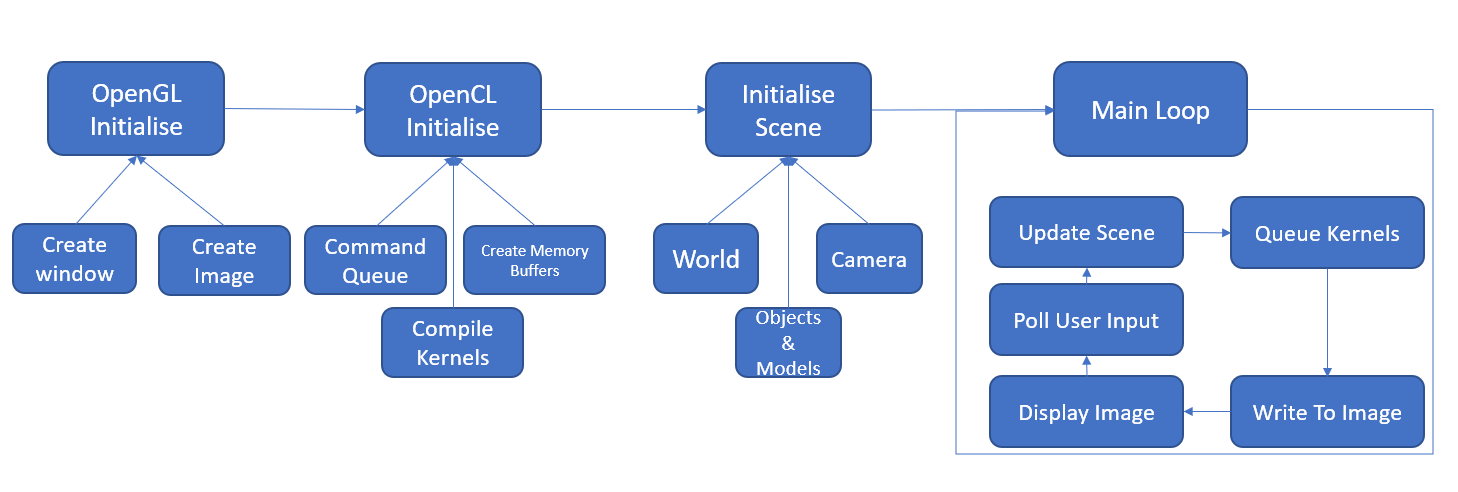
\includegraphics[width=\textwidth]{img/architecture_diagram.png}
    \caption{Diagram of the implementation architecture design}
    \label{arch_design}
\end{figure}

\subsubsection{Host}
% Write about the things that happen on the host side (e.g. creating memory buffers for data, images, etc)
% Main loop, queue and waiting for queue, displaying the results, data transfer

Device memory usage in kernels must be managed by the host because there is no way to dynamically allocate or de-allocate memory in kernels. An alternative to this would be to create new memory buffers on the host side and set a kernel argument to the newly created memory buffer however this is slow and would likely have a significant impact on the time spent in the main loop. Due to the nature of this, the memory usage is generally static and any apparent additions in memory, e.g. adding an object to the scene, is usually a memory update in a pre-allocated memory buffer. For example, the host may pre-allocate a memory buffer large enough to store 1000 spheres so the device program will always be using at least 1000 spheres worth of memory even if the entire memory block are $0's$ or the kernel never uses the memory buffer.

The device also has no control over data transfer between device memory and host memory. The device can read and write memory between device memory in the form of memory buffers however only the host can manipulate data between host memory and device memory. Because of this, there is less flexibility with code in OpenCL.

\subsubsection{Device}
% Write about OpenCL kernels, memory management (e.g. memory types: global, constant, private, local),
% Include limitations of OpenCL CLang, CLang datatypes and unique features

When memory buffers are created via the host, the host must specify an address space in which the memory buffer is created in and can be one of the following: global, local, constant, private. Depending on the OpenCL implementation, the different address spaces could offer major performance benefits and could be physically allocated in different physical memory or memory types. Memory allocated in the constant address space are read-only to kernels and may be cached more aggressively, providing a performance boost to access to the cached memory. Global memory is generally the slowest address space as OpenCL must allow the kernels write access to the memory. Constant and Global memory can be accessed by all work-items of a kernel during its execution however since memory in the constant address space will be unchanging between work-items, its contents can be cached. Local an private memory are generally declared inside the kernel function itself with no interaction with the host. Local memory can be accessed by all work-items in a work-group however private memory can only be accessed by the work-item. To increase access performance, if a kernel requires multiple reads from global memory, it is copied to private memory via code where subsequent accesses to the required data is done via the private copy. Obviously, this solution will provide any performance benefit when writing to global memory. When a memory buffer is shared with the OpenGL context, whenever OpenGL accesses the memory buffer, the data in the buffer will always be up to date as the actual memory on the device that both the OpenCL and OpenGL handles point to are the same. This is evident as the OpenGL image is displayed immediately after the OpenCL kernel responsible for writing to the image memory buffer is executed.

The OpenCL C programming language, while based on C99, has some limitations due to the fact that memory cannot be allocated during kernel execution and functions undergo a similar optimisation to loop-unrolling. As a result, recursive function calls are forbidden and control flow is limited. This poses a problem for recursive ray tracing where the results of the rays traced must be concluded backwards (from the tail end). The workaround used was to use a statically allocated array acting as a heap to process rays in a recursive fashion iteratively. \citep{gaster2012heterogeneous} While there are some limitations and little flexibility, OpenCL C does include some quality of life advantages with built-in functions and data-types that align with the type of processing required by ray-tracing. The built-in functions include \textit{dot}, \textit{cross}, and mathematical functions such as \textit{log} and \textit{sqrt}. Alongside regular scalar data types, OpenCL C also includes vector data types which can conveniently represent data constructs such as positions or directions. I.e. a ray is a structure composed of two \textit{float3} representing the ray's origin and direction.

\subsection{Kernel Structure}
% Write about the kernels that are used and why there are multiple kernels.
% Include file structure and header files usage, order of kernels and kernel dependencies
% Include why monolithic kernels may be bad

Designing a kernel architecture for ray-tracing which takes advantage of multiple kernels is a non-trivial task. While a single monolithic kernel can be used to execute the whole process, from ray-tracing to image and colour processing, it is generally a better idea to separate parts of the process into individual kernels where independent code and relevant memory are isolated \citep{laine2013megakernels}. When code performing independent tasks are separated into individual kernels, the code base is generally more organised easier to refactor if needed. Another benefit is that having multiple kernels naturally encourages vectorisation in the processing of data instead of using branching inside a single kernel. The ray-tracer implementation uses two kernels, a kernel for tracing rays, and a separate kernel for processing the results of the trace and writing the produced colours to the image.

The command queue allows kernels to be queued with $ND$ range where $ND$ represents the dimensions of the range (e.g. 3D for a three dimensional range) and in an $ND$ range kernel execution, each work-item is given $N$ ID's which correspond to the range. E.g. a $2D$ range of $3 \times 3$ will result in $9$ work-items executing the kernel with two ID's ($0, 1, 2$) in each dimension. During kernel execution, the work-item can query its global ID which can be used to access data in locations corresponding to its ID's.

\subsubsection{Ray Trace Kernel}
% Write that the rays are generated here and traced (intersection test with world objects)
% Include that results are saved to a global buffer which will be used in other kernels

The ray-trace kernel is responsible for generating rays and tracing them by running intersection tests with objects in the scene. No colour processing or image generation is executed in this kernel; the kernel only handles tracing rays and storing the results in a memory buffer that will be accessed by a separate kernel to generate the image. The kernel is queued with a $2D$ range of the image resolution width by the image resolution height which will allow for easy method for the work-item to identify which pixel it should trace rays for as the kernel can simply query its global ID's to find which pixel it is for without any additional processing.

Since the image generation is not happening in this kernel, the results produced when the rays are traced must be stored in a memory buffer for a different kernel to use. To store results of a ray that is traced, a C struct was created to encapsulate the data produced such as the intersection point, surface normal, object index, object type. The global memory buffer that acts as storage for the trace result data is an array of the result struct with varying array length depending on the number of bounces and the number of secondary rays that are passed to the other kernel. The array length can be calculated by $W \times H \times N$ where $W$ and $H$ are the width and height of the image and $N$ is the maximum number of rays traced including the primary ray and any subsequent secondary rays. $N$ can be calculated with $$\frac{1 - C^{B+1}}{1-C}$$ where $C$ is the number of child rays (child rays are rays stemming from a primary ray or secondary ray whereas secondary rays are all other rays that are not the primary ray) and $B$ is the number of bounces.
To get the starting index in the array for each pixel, the same formula can be used, replacing $W$ and $H$ with $X$ and $Y$ which are the global ID's in each dimension. The formula is based on the summation formula for geometric progression where the first term is 1 \citep{rosen1999handbook}.

\subsubsection{Image Kernel}
% Write that the image is generated in this kernel. The OpenGL image buffer is written to.
% Include that the data is from the ray trace kernel.

When all the rays have been traced, the information retrieved from the rays can be used to create an image based on the path the ray travelled and the objects it intersects with each bounce. The global memory buffer used in the \textit{ray-trace kernel} is passed to this kernel as an argument as \textit{global} as it is in the global address space however the buffer only needs to be read from in the image kernel. The kernel requires multiple accesses to the global memory buffer and global memory access is slow so the each of the kernel work-items copies a slice of the global memory buffer that it will read from. The image kernel is queued with the same \textit{ND range} as the ray-trace kernel so the global ID's will be the same for the same working pixel and so the formula used to calculate the index offset in the global memory buffer for each work-item is the same; this is used to find the starting location of the slice when copied from the global memory buffer into the work-items own private memory and using $N$, as previously mentioned, for the length of the slice.

A tree is used to structure the rays and their children in the global memory buffer array. The colour result of any ray is dependent on the colour result of all child rays so the kernel must calculate the colour results starting with the deepest node in the tree. Thus, the kernel uses a depth-first approach when traversing the tree. A node's final colour result is a mix of its own material and the colour results of its child rays. If the child index for each type of ray (reflection, refraction, etc) is consistent for each node, then the index of the node can be used to identify its type which affects how the the colour is mixed into the final colour result of the node. If the ray doesn't intersect with an object, it queries a cubemap texture for its result colour based on the ray's direction which represents the sky/environment.

Overall, the only tasks performed in this kernel is to determine the colour of the output based on the materials of the surfaces that the rays intersect. No actual ray-tracing is performed during the execution of this kernel.

\subsubsection{Reset Kernel}
% Write that the results generated in the ray trace kernel are reset here

A third kernel is used during the process to ensure that in the next iteration of the main loop, the working global memory buffer that stores the ray-trace results structs is cleared. The kernel is queued with a 1D range from $0$ to $L$ where $L$ is the length of the global memory buffer. While the result struct is relatively large, not a lot of data must be written as only a single boolean flag must be written to for each member of the array. The purpose of the boolean flag is simply to indicate whether the the ray has been traced as some rays will be omitted if they do not need to be traced. E.g. when the intersecting object material is completely opaque, a refraction ray does not need to be traced. 

\subsubsection{Monolithic Kernel}
% Write that due to memory limitations from the results buffer in the ray trace kernel that a single kernel may be necessary
% Include physical memory limit vs cl_mem buffer allocation limit

If a single kernel is used for the entire process, the need to store data into a global memory buffer is removed as the work-item will have all the data necessary and the data will be encapsulated within the work-item. The only memory buffers that need to be created on the host side will be the scene objects and the final image output. The storage for the ray-trace data will be local variables inside the kernel because there is no need for access to the ray-trace data outside of the kernel. 

Depending on the hardware, there is also a limitation on the size of memory buffers less than the total memory of the device. If the bounce limit was too high or the number of child rays was too high, the size of the global memory buffer may be higher than the limit and would prevent the buffer from being created. However there is not a limit to the number of local variables in a work-item (or the limit is sufficiently large) and the size of the array would be substantially less as it only has to contain the data required for a single work-item, much less than a single buffer for the entire image.

This kernel structure is not encouraged \citep{laine2013megakernels} as it naturally results in less organised code, maintainability, and may result in a lower performance. There is also less flexibility on profiling and event control as the entire ray-tracing to image process becomes one single event on the command queue.

\subsection{Ray Generation}
% Mention only basic rays will be included in this section. <-- no
% Talk about backward ray tracing

In the ray-trace kernel, rays are generated by computing their origins and directions with each intersection or by the view in the case of primary rays. Unlike the real world, the rays will originate from the view/eye and be traced outwards; this is backward ray tracing. The method of computing the starting position and direction of a ray differ with the intersect surface material. Typically, a child ray's origin is the at the intersection point of the parent ray and the direction is some function of the parent ray direction.

In most cases, the secondary rays will have to go through all the same scene intersection tests as the primary ray and may even have to perform extra computation for its specific needs when traced.

\subsubsection{Primary Rays}
% Talk about eye rays, method of generation. Explain there's a ray for each pixel. Include diagram and pseudocode
% Explain camera movement here (rotation and translation). Include normalisation (pixel coord for ray position and direction)

With the pixel coordinates specified by the kernel global ID's, the normalised ray origins are computed with:

\begin{align}
    N &= \begin{bmatrix}
        (2(x / w) - 1) * r \\
        2(y / h) - 1 \\
        D
    \end{bmatrix}
\end{align}

where $x$ and $y$ are the pixel coordinates, $w$ and $h$ are the image width and height, $r$ is the aspect ratio (height/width), and $D$ is the distance Z-axis offset of the ray origin to the camera position.

Since the camera can move and rotate, primary rays will vary depending on the rotation angle and the camera position. The ray origin can simply be offset by the camera position for translation. For rotation, given the vertical and traversal axis angles, the ray direction is computed by 
$$[ N_x, N_y * cos(a) + N_z * -sin(a), N_z * cos(a) + N_y * sin(a) ]$$ where $N$ is the normalised coordinates of the pixel and $a$ is the traversal axis angle of the camera rotation (pitch). The vertical axis angle (yaw) can then be applied with $$[ O_x * cos(b) + O_z * sin(b), O_y, O_z * cos(b) + O_x * -sin(b) ]$$ where $O$ is the position vector returned by the traversal axis angle formula.

The ray direction is computed by simply taking the normalised vector of the camera position to the ray origin.

\begin{figure}
    \centering
    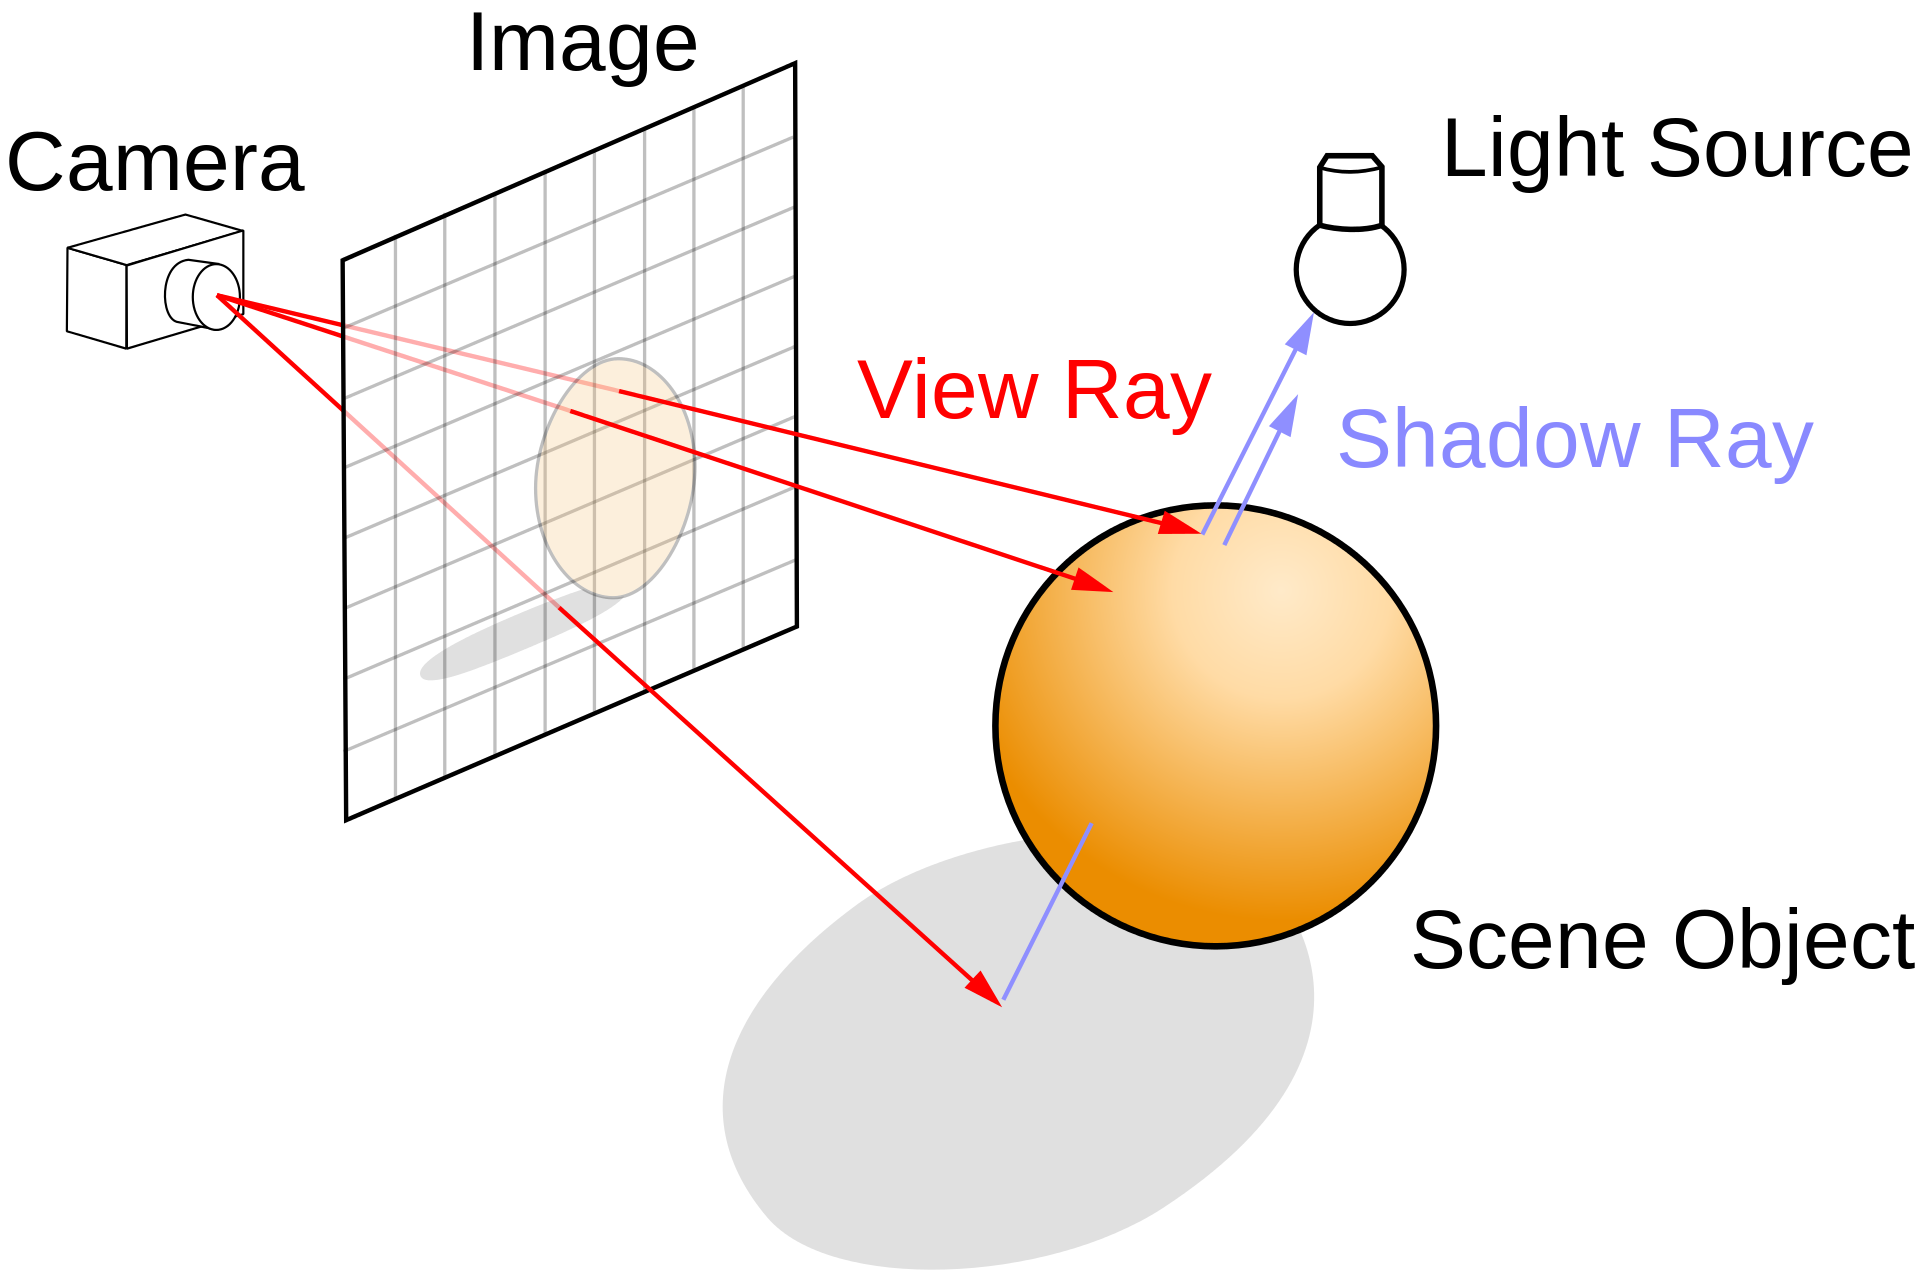
\includegraphics[width=\textwidth]{img/backward_ray_tracing.png}
    \caption{Diagram of how primary rays are generated from the camera. \citep{henrikdia}}
\end{figure}

\subsubsection{Reflection}
% Write about generating reflection rays using the normal of primary ray result. Use pseudocode and diagram.
% Mention secondary rays and recursion

When a ray hits a surface and the surface material is reflective, a child ray for reflection is created. The origin of the reflection ray is the intersection point of its parent ray and the direction of computed by $$I - 2N(I \cdot N)$$ where $I$ is the parent ray direction, $N$ is the surface normal, and the dot represents the dot product. The result of the reflection ray will be mixed into the output result of its parent ray depending on the surface material. If a ray does not intersect with any object or the surface material is not reflective, a reflection ray is not generated. When a reflection ray intersects with an object, it may create a child ray of itself for another reflection ray depending on the bounce limit. The rays can be traced sequentially however the colour results must be computed in a recursive manner to be physically accurate.

\begin{figure}
    \centering
    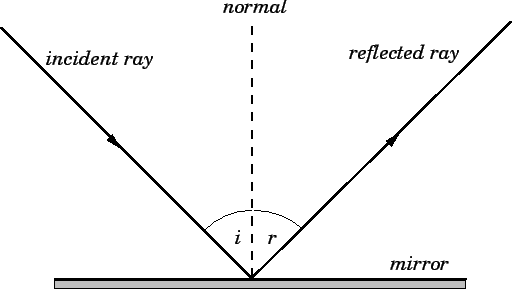
\includegraphics[width=\textwidth]{img/reflection_diagram.png}
    \caption{Diagram of how the reflection direction vector is computed. \citep{fitzpatrickreflect}}
\end{figure}

\subsubsection{Refraction}
% Same as reflection

If the ray hits a surface that is not completely opaque, like the reflection ray, a child ray is created for refraction transmission. Similar to reflection, the origin is at the intersection point and the surface normal is used to compute the direction of the refraction ray. The refraction ray will usually be traced through the object that was hit. In order to compute the direction, the refractive indices of the parent ray medium (e.g. air) and object are needed. The following pseudocode is how the refractive direction is computed in the kernel.

\begin{algorithm} [H]
\SetAlgoLined
\KwResult{Direction of the refraction ray: $R_d$}
\KwData{
I = incident direction vector, 
N = surface normal, 
F = previous medium refractive index, 
T = object medium refractive index
}

$n = F / T$ \\
$C = -N \cdot I$ \tcp{Dot product} 
$S = n^2(1 - C^2)$ \\
\tcp{Total internal reflection} 
\uIf{S > 1}{return} 
$T = \sqrt{1 - S}$ \\
$R_d = n \times I + n(nC - T)$


\caption{Algorithm to compute the refraction direction of a given incident direction and surface normal.}
\end{algorithm}

When total internal reflection occurs, the refraction ray is ignored. In most cases, the refraction ray will intersect a surface of the same object (the refraction ray travels through the object) where another refraction ray would be generated, this time from inside the object going away from the object. The $F$ and $T$ values will be opposite in this case compared to the previous refraction computation.

\subsubsection{Shadows}
% Write how shadows work
% Why it's not perfect (depends on light source)
% Soft shadows

Because rays are traced backwards (from the camera towards light sources), surfaces in shadows need to be calculated differently. In the physical world, there is simply less light coming the surface so it appears darker. However due to the nature of backward ray tracing, a shadow ray is created and traced towards a light source where the surface is in shadow if the shadow ray intersects with any object.

Shadows traced this way will produce very hard shadows where the edges of the shadow will follow very close to the edges of the object which will look unrealistic due to global illumination from light bouncing around in the real world where parts of the shadowed surface will be illuminated by light bouncing off objects nearby. The effects of the hard shadow edges can be mitigated by tracing multiple shadow rays with a slight offset towards the same light source and the strength of the shadow for a particular point on the surface is calculated with $\frac{H}{N}$ where $H$ is the number of shadow rays that have hit an object and $N$ is the total number of shadow rays traced.

This approach of creating shadows is less physically accurate and shows in the image produced as surfaces that are not completely opaque will not let light through like it would in the real world without tracing even more rays and including refraction. With soft shadows, including this feature would hinder performance too much.

\begin{figure}
    \centering
    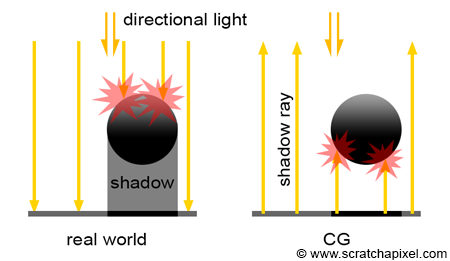
\includegraphics[width=0.5\textwidth]{img/shadow_diagram.png}
    \caption{Diagram of shadow rays \citep{scratchshadow}}
\end{figure}

\subsection{Intersection With Objects}
% Write that for an image to be produced, the ray needs to hit an object and return a value
% So explain why we need intersection

To produce an image, the rays traced must return information that can be used to compute the result colour of the ray and be mixed to produce the final output colour of a pixel. The information information returned is based on the surface material of the objects that are hit by the rays. The surface material includes information such as diffuse colour, opacity, reflectance, and refractive index of the object medium.

\subsubsection{Sphere Intersection}
% Use pseudocode and diagram and sphere struct
% Include which secondary rays are generated as a result

Ray intersection with spheres are simple and quick. A sphere is stored in memory as a C struct containing its position, radius, and material. For better memory efficiency, the material is stored as an index to a separate material buffer as many objects may use the same material. Sphere intersection is calculated with the following pseudocode.

\begin{algorithm}[H]
    \SetAlgoLined
    \KwResult{True if ray intersects sphere, else false}
    \KwData{Ray $R$, sphere position $S_o$, sphere radius $S_r$}

    \tcp{Parametric equation: $at^2 + bt + c = 0$}
    $b = 2(R_d \cdot (R_o - S_o))$ \tcp{Dot product}
    $c = (R_o - S_o)^2 - S_r^2$ \\
    \uIf{$b^2 - 4c < 0$}{return false}
    $d = \sqrt{b^2 - 4c}$ \tcp{Discriminant}
    $T_{min} = (-b - d) / 2$ \\
    $T_{max} = (-b + d) / 2$ \\

    return true

\caption{Procedure used to determine if a ray intersects with a sphere.}
\end{algorithm}

$T_min$ and $T_max$ can be used to find the intersection points of the sphere. The ray does not intersect with the sphere if the discriminant is negative. The normal of the surface is simply the vector from the sphere center to the surface intersection point.

\subsubsection{Triangle Intersection}
% Write about versatility of triangles and how models use them (the reason we use triangles)
% Include that it is relatively slow for complex models with lots of triangles
% Include that there are methods to get around performance issues
% Include diagrams and pseudocode

While spheres are simple and quick, they are not the most versatile shape for complex objects. Any 3D model can be represented as a triangular mesh so a ray-triangle intersection test was also implemented. Triangle intersection tests are slower than sphere intersections and 3D models can have a performance crippling number of triangles to test however there are methods to reduce the number of triangles a ray needs to test for intersection.

\begin{algorithm}[H]
    \SetAlgoLined
    \KwResult{True if ray intersects triangle, else false}
    \KwData{Ray $R$, Triangle vertices $V1, V2, V3$}
    $edge_1 = V2 - V1$ \\
    $edge_2 = V3 - V1$ \\
    $h = R_d \times edge_2$ \tcp{Cross product}
    $a = edge_1 \cdot edge_2$ \\
    \tcp{If ray is parallel to triangle}
    \uIf{a = 0}{ return false}
    $f = 1 / a$ \\
    $s = R_o - V1$ \\
    $u = f(s \cdot h)$ \\
    \uIf{$u < 0 \; OR \; u > 1$}{ return false }
    $q = s \times edge_1$ \tcp{Cross product}
    $v = f(R_d \cdot q)$ \\
    \uIf{$v < 0 \; OR \; v > 1$}{return false}
    $t = f(edge_2 \cdot q)$ \\
    \tcp{If triangle is behind ray origin}
    \uIf{$t < 0$}{return false}
    return true

    \caption{Ray Triangle Intersect}
\end{algorithm}

\subsubsection{OBJ Models}
% Write how 3d models are loaded
% Write how models are composed of triangles
% Write briefly how rendering can be slow if a model has many triangles

3D models are stored in files in OBJ format with a list of vertices, list of normals, and list of faces where each face will have the indices of the vertices and normals. The OBJ files are loaded and parsed on the host and converted into a similar format designed for the kernels to use. A separate buffer is created to store the vertices, normals, and faces of every model and triangle which are passed to the kernels as kernel arguments. Models with many triangles will largely affect the intersection time as the rays will test intersection with every triangle without acceleration structures.

\subsection{Generating An Image}
% Write how you need to mix light from the different rays to generate the final colour
% Using material information (mention material properties like opacity, reflectivity, diffuse)

The resulting light output from all of the secondary rays must be mixed to generate the final colour and output of the primary ray. Depending on the surface material properties (opacity, reflectance, etc), mixing the colours of the child rays will be different. The output result colour must be processed from the tail-end of the result stack as a parent ray must use the result of its child rays to produce its own output.

\subsubsection{Phong Model}
% Write about base colour from only primary ray
% Not most realistic but quick and convenient
% Basic shading/lighting
% Include picture

The base colour output from when a ray intersects with an object is computed using the Phong model where the surface material's ambient, diffuse, and specular values are used. If the material is not reflective, completely opaque, and not in shadow, this will be the colour output for the ray. While not completely physically accurate, it provides a rough estimate of the shading and lighting of the object and is relatively fast \citep{bishop1986fast}. The Phong output will be combined with the other child ray outputs if the surface material allows it which may produce a better result. Algorithm \nameref{phongalgo} is used to compute the Blinn-phong colour output in the kernel \citep{blinn1977models} which is a faster Phong approximation algorithm and can be more accurate in some cases.

\begin{algorithm}
    \label{phongalgo}
    \SetAlgoLined
    \KwResult{Colour output computed with Phong}
    \KwData{$A, D, E, R, N, L$}
    \tcc{
        $A$: Ambient, $D$: Diffuse, $E$: Specular Exponent, $R$: Ray, $N$: Surface Normal, $L$: Light Direction
    }

    $I = N \cdot L$ \tcp{Light intensity}
    $C = I \times D$ \tcp{Diffuse colour}

    $H = normalize(L + R_d)$ \tcp{Blinn-Phong Half Vector}

    $I = (-N \cdot H)^E$ \tcp{Specular colour intensity}

    return $A + C + I$
    
    \caption{Compute Phong Colour}
\end{algorithm}

Figure \ref{phong_img} shows a non-reflective and opaque object in the scene with its colour output computed using the Phone model.

\begin{figure}
    \centering
    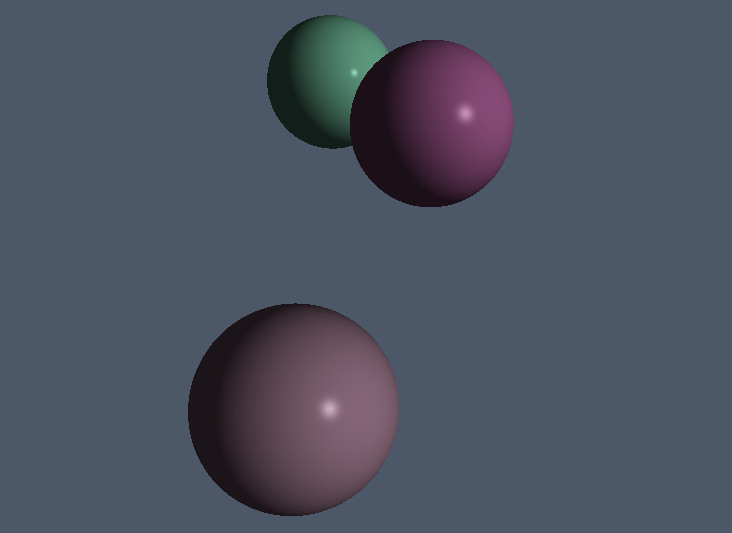
\includegraphics[width=\textwidth]{img/phong.png}
    \caption{Sphere with Phong shading}
    \label{phong_img}
\end{figure}

\subsubsection{Transmission \& Reflection}
% Write about how the transmission colour is generated based on material (opacity etc)
% Write about how the reflection colour is calculated (reflectivity)
% Show picture of refraction by itself and reflection by itself
% Include picture with different refractive indices

The final output of a ray hitting a surface is simply a mixture of the reflection, shadow, and transmission. The transmission itself is a mix of the base material colour (Phong) and the light output of any rays that go through the object (refraction). When opacity is less than $1.0$ ($0.0$ is fully transparent and $1.0$ is fully opaque), refraction rays are traced and the result is linearly mixed with the base colour based on the opacity.

If a ray does not intersect with any object, the output becomes the background or sky colour dependent on the ray direction and there are no child rays created. Similarly, if the ray has reached the bounce limit, no child rays will be created for that ray. 

Transmission for any ray is computed with $mix(refract, base, opacity)$ where the $mix$ function is a linear interpolation function, $refract$ is the colour output of the refract child ray, and $base$ is the base colour computed by the Phong model. If the ray has reached its bounce limit and does not have a refract child ray, the opacity is simply treated as $1.0$.

If a reflect child ray has been traced, the colour output of the reflect ray is mixed with the transmission based on a Fresnel factor which will be discussed in the next section.

Figure \ref{sphere_reflect} shows a fully opaque sphere with 100\% reflectance.

Figures \ref{sphere_refract_solid} and \ref{sphere_refract_hollow} show a fully transparent sphere with refractive index $1.157$ and $1.04$. For demonstration purposes, the spheres are shown with reflection omitted to only show the effects and results of refraction. Comparing the images, the amount the refractive index changes the direction of the refraction ray is clear.

Figure \ref{spheres_refractive_index} shows a lineup of transparent spheres with varying refractive indices.

\begin{figure}
    \centering
    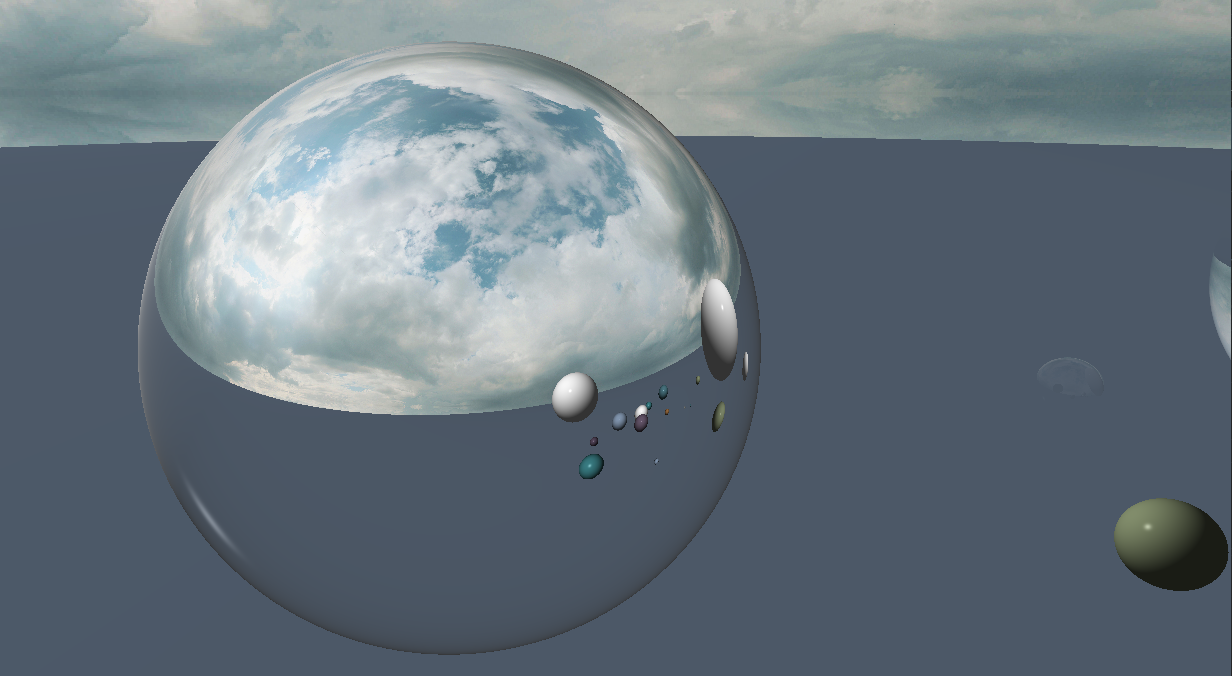
\includegraphics[width=\textwidth]{img/reflection.png}
    \caption{Sphere with reflective material}
    \label{sphere_reflect}
\end{figure}

\begin{figure}
    \centering
    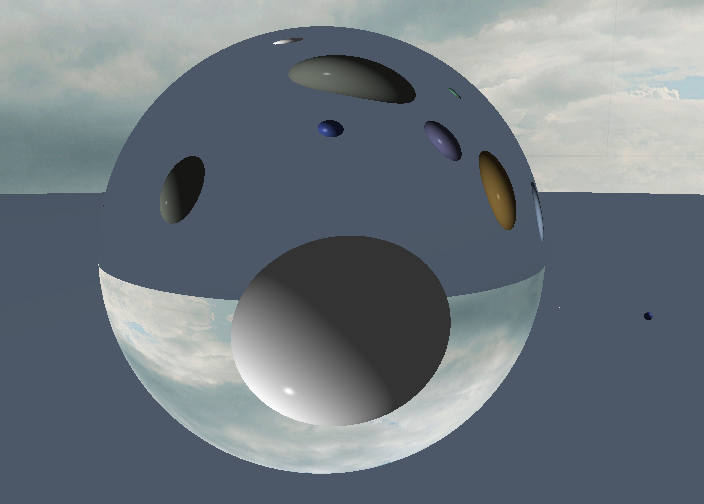
\includegraphics[width=\textwidth]{img/refraction_solid.png}
    \caption{Sphere with transparent material with refractive index 1.517}
    \label{sphere_refract_solid}
\end{figure}

\begin{figure}
    \centering
    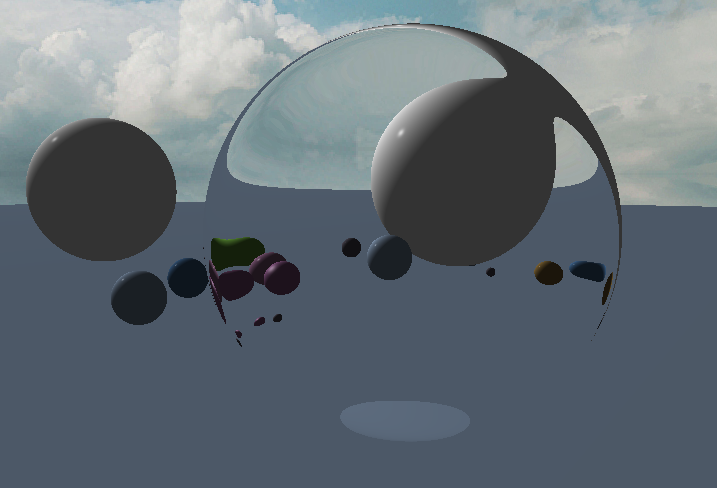
\includegraphics[width=\textwidth]{img/refraction_hollow.png}
    \caption{Sphere with transparent material with refractive index 1.04}
    \label{sphere_refract_hollow}
\end{figure}

\begin{figure}
    \centering
    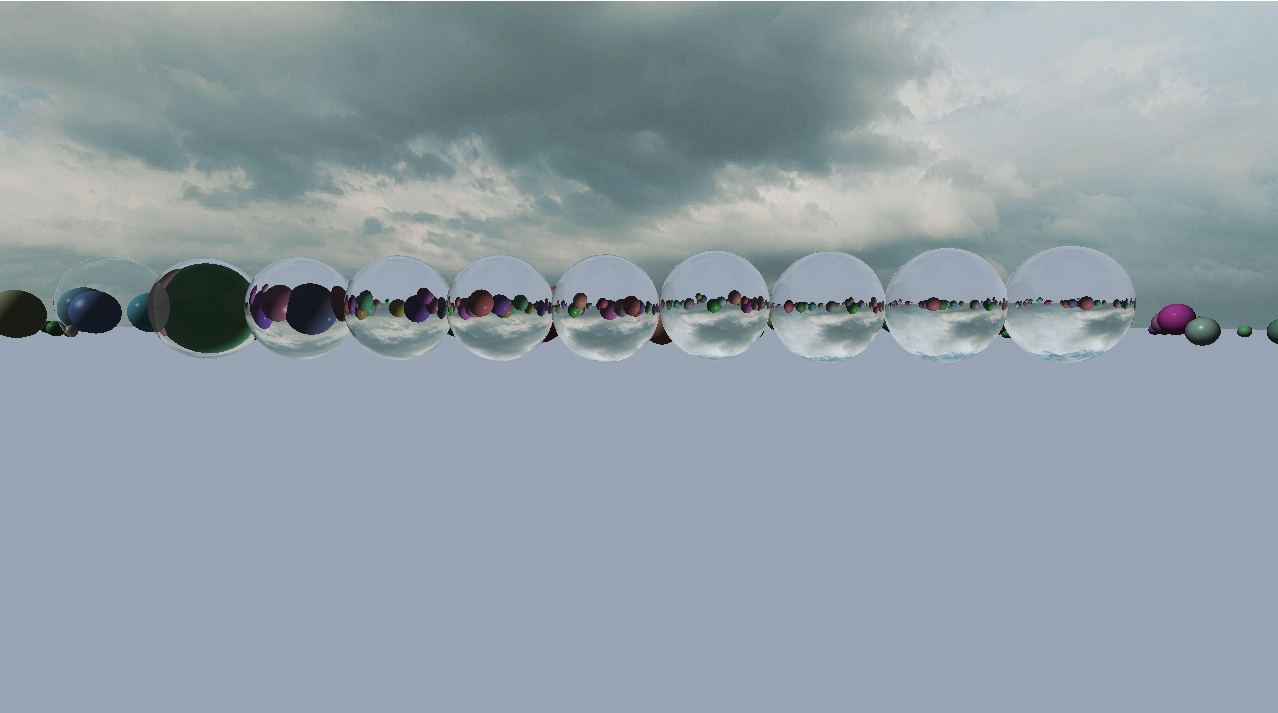
\includegraphics[width=\textwidth]{img/refractive_index.png}
    \caption{Spheres with increasing refractive index ranging from 1.0 -> 1.7}
    \label{spheres_refractive_index}
\end{figure}

\subsubsection{Fresnel}
% Write how real world material is a mix of refract and reflect
% Linear mix is not correct
% Include algorithm and how it affects reflection and transmission amount
% Include picture of fresnel effect with both refraction and reflection

For accurate results, a transparent material such as glass should use a mix of both the transmission and reflection light however a linear mix is simply not accurate. A more physically accurate approach uses a factor based on the angle of incidence of the ray onto the surface. The transmission factor increases when the angle of incidence increases. With a fresnel factor of $F$, the surface can be coloured with $T(1 - F) + LF$ where $T$ is the transmission colour, $F$ is the fresnel factor (a value $0.0 \rightarrow 1.0$), and $L$ is the reflection colour. The algorithm \nameref{fresnelalgo} shows the implementation of how the fresnel factor is computed in the kernel. Figures \ref{fresnel_solid} and \ref{fresnel_hollow} show the same transparent refractive spheres with mixed reflection using the fresnel factor.

\begin{algorithm}
    \label{fresnelalgo}
    \SetAlgoLined
    \KwResult{Fresnel Factor}
    \KwData{$I, N, F, T$}
    \tcc{$I$: incidence direction vector, $N$: surface normal, $F$: refractive index of the ray medium, $T$: refractive index of the object medium}

    $cosI = I \cdot N$ \\
    $n = \frac{F}{T}$ \\
    $sinT = \sqrt{n * (1 - cosI^2)}$ \\
    $cosT = \sqrt(1 - sinT^2)$ \\
    $R_s = \frac{TcosI - FcosT}{TcosI + FcosT}$ \\
    $R_p = \frac{FcosI - TcosT}{FcosI + TcosT}$ \\
    return $\frac{R_s^2 + R_p^2}{2}$ \\

    \caption{Function for computing the fresnel factor}
\end{algorithm}

\begin{figure}
    \centering
    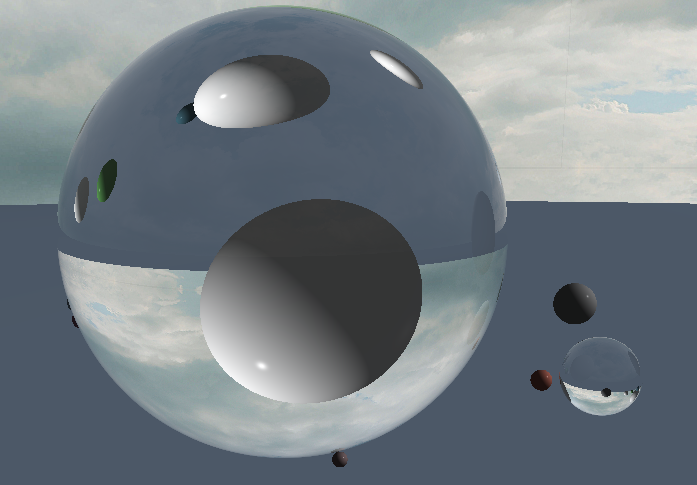
\includegraphics[width=\textwidth]{img/fresnel_solid.png}
    \caption{Transparent sphere with refractive index 1.517 with fresnel effect}
    \label{fresnel_solid}
\end{figure}

\begin{figure}
    \centering
    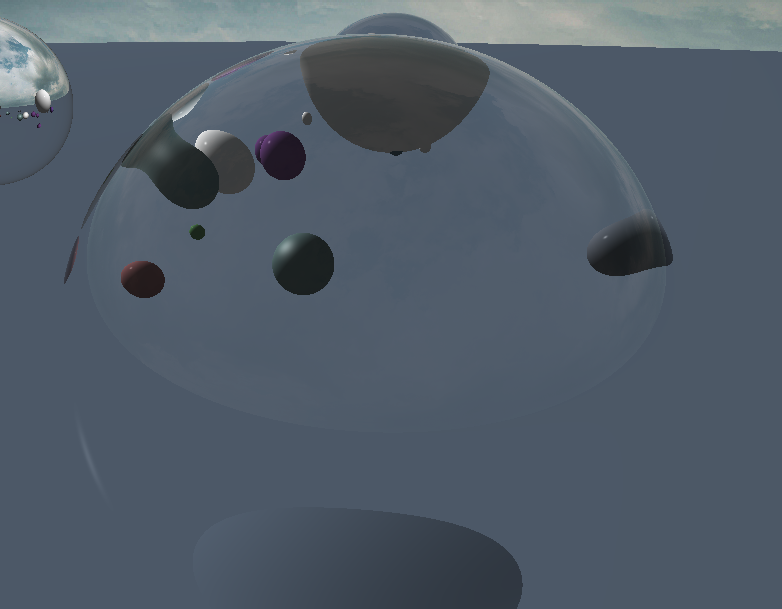
\includegraphics[width=\textwidth]{img/fresnel_hollow.png}
    \caption{Transparent sphere with refractive index 1.04 with fresnel effect}
    \label{fresnel_hollow}
\end{figure}

\subsubsection{Shadows}
% Write how shadows reduce the light depending on whether the shadow ray intersects or not.
% Not physically accurate as the light is subtracted rather than just not added
% Write how light is reduced by a factor
% Write about how soft shadows work, multiple shadow rays etc
% More shadow rays = less performance
% Write how low amount of rays don't impact performance that much (INCLUDE HOW THERE'S NO MEMORY OVERHEAD)
% How small shadow distance with low shadow rays can have an anti-aliasing effect even if it's not soft
% Include shadow picture
% Include soft shadow picture

The implementation of shadows reduce the light or colour intensity of the surface instead of the more physically accurate approach where light simply does not bounce on shadowed surfaces as much. If the shadow ray created with an origin at the surface intersects with an object, the surface is simple treated as in shadow. A surface is either in shadow or not in shadow and this boolean flag will determine whether the surface light intensity needs to be reduced or not. Surfaces in shadow are simply reduced by a fixed factor. This approach produces hard shadows as seen in figure \ref{hard_shadow}.

The performance impact is trivial however it does not produce results that are physically accurate or realistic. For softer shadows, multiple shadow rays can be traced to determine the strength of the shadow at a particular spot on the surface. The extra shadow rays have their origin offset by a small distance, still directed at the light source. Shadow rays near the edge will have a larger disproportion between shadow rays that intersect and rays that don't intersect. To make the surface shadow softer, the amount the intensity is reduced is lessened by the proportion of missed shadow rays to hit shadow rays. The more extra shadow rays are traced, the smoother the shadow.

When only using a few extra shadow rays, the soft shadow effect only gives it a slight anti-aliasing effect which may be beneficial and only impact performance slightly.

Figures \ref{softish_shadow} and \ref{soft_shadow} show the shadow with varying level for softness.

\begin{figure}
    \centering
    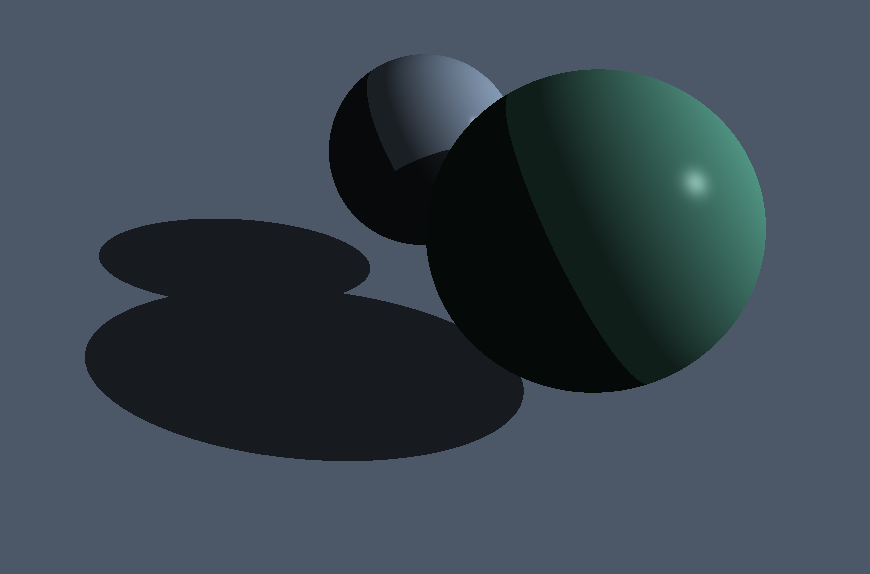
\includegraphics[width=\textwidth]{img/hard_shadow.png}
    \caption{Sphere casting a hard shadow on a surface}
    \label{hard_shadow}
\end{figure}

\begin{figure}
    \centering
    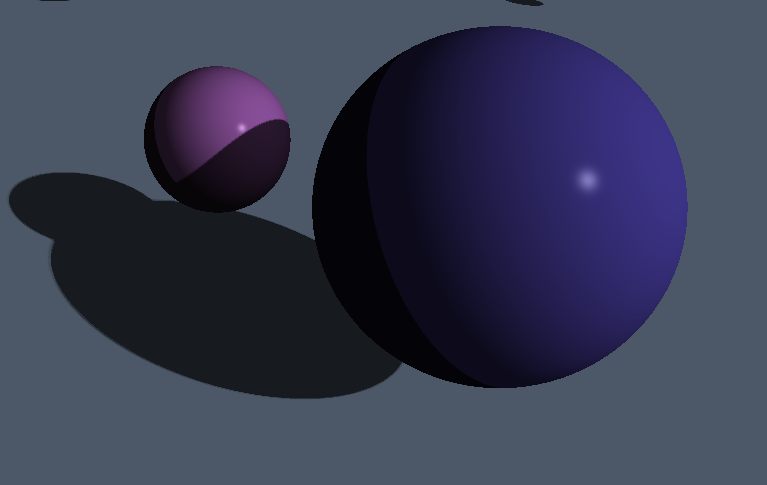
\includegraphics[width=\textwidth]{img/softish_shadow.png}
    \caption{Shadow with anti-aliasing}
    \label{softish_shadow}
\end{figure}

\begin{figure}
    \centering
    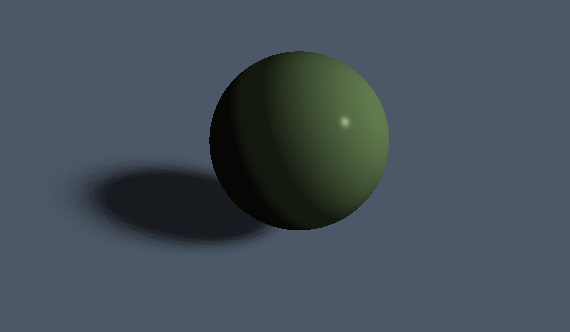
\includegraphics[width=\textwidth]{img/soft_shadow.png}
    \caption{Sphere casting a soft shadow on a surface}
    \label{soft_shadow}
\end{figure}

\subsubsection{Combining Secondary Rays}
% Write how because of backward ray tracing the correct method would be recursive
% Write about limits of OpenCL recursion
% Write how a stack and array is used as a replacement

For accurate compution of a ray's output, the output of its child rays must be resolved first. This can usually be achieved by running the colour compution procedure recursively on each of the rays children before computing the rays own output however recursion is not supported in the OpenCL kernel language. The alternative method implemented a workaround to recursion by using an array as a stack. Since dynamic arrays are also not supported, a static array with a maximum size limit was used with a variable to keep track of the stack head which represents the index of the static array which is free and a variable to keep track of the recursive traversal through the stack. The recursive function approach would have called the function recursively multiple times so the stack must represent a tree with $N$ children where $N$ is the number of child rays that can be generated off a single ray.

\subsection{Acceleration Structures}
% Write about how the majority of the time taken during the rendering process are the ray intersection tests
% Mention how a naive approach would be to intersect test on every single object, sphere, triangle etc
% Use some example numbers to show how many number of tests total there would be
% The best way to reduce the time spent on rendering is reducing the number of tests
% Could also optimize the intersection algorithms although this would have less impact that reducing rays
% Acceleration structures are used to decrease the amount of intersection tests a ray needs
% A perfect method would make it so the ray only tests against objects that it will definitely intersect with
% Obviously this is not reasonable but it is the target of the acceleration structures

The majority time taken during the rendering process is in the ray intersection tests. The naive approach is testing for intersection between a ray and every object in the scene however this is inefficient and some faster preliminary checks can be made to reduce the number of ray-primitive intersection tests. For example, a $1280 \times 720$ image with a single sphere taking up $200 \times 200$ pixels on the image need only perform ray-sphere intersection $40000$ times instead of the full $921600$ times if every primary ray were to perform the intersection test. However if the object were to take 100\% of the screen space, the preliminary checks may end up negatively impacting performance (although slight). Fortunately this is hardly ever the case during a typical scene.

Another way to improve render time is to optimise the intersection algorithms although this would have less impact than just reducing the number of tests. The acceleration structures: bounding volumes and grid, are used to reduce the number of intersection tests by omitting them from rays which can be determined to not intersect with the object without doing an intersection test. A perfect method would have rays only perform intersection tests with objects that it does intersect with however obviously this is farfetched and unreasonable but it is the target of acceleration structures.

\subsubsection{Preliminary Checks}
% Write how you can do some simple checks for objects with a large number of triangles if they are definitely not intersecting (e.g. radial checks)
% Algorithm optimizations in sphere tests
% Write how this wouldn't improve things when the prelim checks pass and the ray would still have to intersect with the rest of the object
% This also won't solve problems if there are lots of individual objects as there would still be a lot of preliminary checks

There are some simple checks that can be performed for objects with large number of triangles such as radial checks or AABB checks however some models and shapes may not make the best use of the area that is checked with these methods. For this reason, models are checked with a bounding volume. For spheres, before the intersection is performed, a simple dot product check is performed so the intersection test is skipped if the sphere is behind the ray. The preliminary checks do not have any improvement to performance of an individual ray if the ray does actually intersect with the object as the actual ray-primitive check will still be performed on top of the preliminary check if the preliminary check passes. Additionally, the preliminary checks, while fast, still take a non-zero amount of time and will still be slow when the number of objects is large.

\subsubsection{Bounding Volumes}
% Write how a bounding volume is created for 3d models with lots of triangles
% Write how it is efficient and more precise
% Similar to AABB but on 3 more axis
% Use some numbers to show percentage of reduced intersection tests compared to just brute force (all)
% Show some pictures of the bounding volume
% Include some code for how the bounding volume is generated

Bounding volumes work similar to AABB, checking for overlaps in the bounds of the $X, Y, Z$ axis. Bounding volumes aim to achieve closer bounds to the convex hull while still being computationally inexpensive. This is achieved by using the $X, Y, Z$ axis and an additional $4$ axis which cut the bounds in the diagonal. The axis are defined by: $(S, S ,S), (-S, S ,S), (-S, -S, S), (S, -S, S)$ where $S$ is defined by $\frac{\sqrt{3}}{3}$.

\subsubsection{Grid}
% Write that an efficient algorithm of stepping through a grid
% Only test triangles that are in the grid cells that the ray steps through
% Write how the grid is generated on Host side (CPU side) where an octree is generated first to accelerate the grid generation with the model to improve load times
% Where only the bottom level leaf nodes are added to the grid

\subsubsection{Bounding Volume Hierarchy}
% TODO

\section{Results and Testing}
% To test the real-time performance
% Test correlation between different variables and factors and performance
% To show and test how effective the individual acceleration structures are
% To show how the performance varies between different hardware

\subsection{Ray Intersection Tests}
% Write how the ray intersection tests are executed the most and so should take the most time during the performance profiling.
% Use min max avg

\subsubsection{Ray Tracing with no objects}
% Show performance and ray trace time for no objects as a baseline result

\subsubsection{Ray Tracing Spheres}
% Show performance of spheres with varying number of spheres

\subsubsection{Ray Tracing Triangles}
% Show performance with varying number of triangles in the form of models

\subsubsection{Acceleration Structures}
% Show performance difference with the models but with acceleration structures

\subsection{Resolution}
% Test performance with resolution
% Note how less resolution means less primary rays

% Overall write about the effectiveness of acceleration structures and that they make the most difference
% Explain that there is a correlation (inverse) between the performance and number of objects on the screen
% Which obviously there is a direct correlation between number of intersection tests and objects on the screen

\section{Future Work}
% Write about how a lot more work can be done to improve real-time performance including more efficient algorithms of detecting different shapes instead of relying on triangles only for complex shapes and models
% Also write about improvements to performance by spreading the workload onto the work items more efficiently since the work items that pass preliminary checks and bounding volume checks do a lot more work that rays that just hit the sky/background and terminate.
% How in OpenCL there are a smaller number of work items and work groups that the number of rays so the work-item ray distribution can be improved to get a more stable and steady performance
% More can be done to improve the visual quality of the image as well
% Write about the features that can be added to improve visuals
% Also write about how OpenCL is being abandoned by both AMD and NVidia (the 2 largest GPGPU producers) for a different standard (AMD) and a proprietary standard (NVidia). So development tools are being less actively used and supported.
% Write how this was experienced during the progress of this project. That debugging tools for OpenCL were no longer availabe (AMD APP SDK).
% And OpenCL implementations are different depending on vendor and machine. So that kernel code on one machine behaved differently on another machine (AMD vs Intel). Solution to this may be to use a standard with only 1 vendor (CUDA, RTX) or a newer standard (Vulkan) or (Radeon Open Compute ROCm) which has active developers and better tools however only available on Linux.
% All of the above have pros and cons like platform independence.

\section{Conclusion}
% Write about the importance of acceleration structures
% Write how ray tracing would be a viable approach to producing high visual quality and physically realistic visual effects like reflection and refraction and lighting

\nocite{*}

\newpage
\bibliography{paper}

\end{document}